\documentclass[xcolor=table,dvipsnames]{beamer}

\usepackage{lscape, amsmath, amsfonts, amssymb, setspace, theorem, wrapfig, graphicx, float, multirow, subfig, color, rotating, multicol, datetime, natbib, venndiagram, pstricks, xkeyval, tikz, etoolbox, verbatim}

\usepackage{listings}
\usepackage{xcolor}
 
\definecolor{codegreen}{rgb}{0,0.6,0}
\definecolor{codegreengray}{rgb}{0,0.4,0}
\definecolor{codegray}{rgb}{0.5,0.5,0.5}
\definecolor{codeblue}{rgb}{0.00,0,0.82}
\definecolor{backcolour}{rgb}{0.95,0.95,0.92}
 
\lstdefinestyle{mystyle}{
    backgroundcolor=\color{backcolour},   
    commentstyle=\color{codegreengray},
    numberstyle=\tiny\color{codegray},
    stringstyle=\color{codegreen},
    basicstyle=\ttfamily\footnotesize,
    breakatwhitespace=false,         
    breaklines=true,                 
    captionpos=b,                    
    keepspaces=true,                 
    numbers=left,                    
    numbersep=5pt,                  
    showspaces=false,                
    showstringspaces=false,
    showtabs=false,                  
    tabsize=2
}
 
\lstset{style=mystyle}

\title{GV300 - Quantitative Political Analysis}
\subtitle{University of Essex - Department of Government}
\date{Week 18 -- 27 January, 2020}				% or you can specify a date, just write it down instead of "\today"
\author{Lorenzo Crippa} 

\usetheme[progressbar=frametitle]{metropolis}
\usecolortheme{seahorse}						% try others: wolverine; crane...


\begin{document}
\frame{
\titlepage
}

\frame{
\frametitle{What are we doing today?}
Today's session:
\begin{enumerate}
\item Robust estimation and Generalized Least Squares (GLS)
\item Non-parametric tests
\end{enumerate}
}

\section{Robust estimation and Generalized Least Squares (GLS)}

\begin{frame} 
\frametitle{The importance of constant variance for OLS}
Remember vcov matrix, OLS estimates of parameters and S.E.:
$$\mathbf{\hat{\beta}}= (\mathbf{X'}\mathbf{X})^{-1}\mathbf{X}'\mathbf{Y}$$
$$\hat{\sigma}^2=\frac{\mathbf{\hat{u}}'\mathbf{\hat{u}}}{N-K-1} $$ 
$$\widehat{Var}(\mathbf{\hat{\beta}}) = \hat{\sigma}^2(\mathbf{X'X})^{-1}$$ \pause
\textbf{Assumption 5: Homoscedasticity and no serial correlation}
\begin{enumerate}
\item $Var(u_i|\mathbf{X})=\sigma^2$ for $i=1,2,\ldots,N$ \pause
\item $Cov(u_i,u_j|\mathbf{X})=0$ for all $i\neq j$ \pause
\end{enumerate}
What if we have heteroscedasticity and/or serial correlation or autocorrelation? 
\end{frame}

\begin{frame}[fragile]
\frametitle{Some matrix algebra}
Let's work on the vcov matrix:
\begin{equation}
\begin{aligned}
\widehat{Var}(\mathbf{\hat{\beta}}) \\
& = \hat{\sigma}^2(\mathbf{X'X})^{-1} \\
& = \hat{\sigma}^2(\mathbf{X'X})^{-1} \mathbf{X}'\mathbf{X} (\mathbf{X}'\mathbf{X})^{-1} \\
& = (\mathbf{X'X})^{-1} \mathbf{X}'\hat{\sigma}^2 \mathbf{I}\mathbf{X} (\mathbf{X}'\mathbf{X})^{-1} \\
& = (\mathbf{X'X})^{-1} \mathbf{X}' E(\mathbf{\hat{u}}\mathbf{\hat{u}}'|\mathbf{X}) \mathbf{X} (\mathbf{X}'\mathbf{X})^{-1}
\end{aligned}
\end{equation} \pause
With:
$$E(\mathbf{\hat{u}}\mathbf{\hat{u}}'|\mathbf{X})=
\left[
\begin{array}{cccc}
\hat{\sigma}^2 & 0  		& \ldots & 0\\
0 		 & \hat{\sigma}^2 & \ldots & 0\\
\vdots 	 & \vdots 	& \ddots & \vdots\\
0 		 & 0		& \ldots & \hat{\sigma}^2 
\end{array}
\right] = \hat{\sigma}^2 \mathbf{I} = \Sigma
$$ \pause
Problem with heteroscedasticity: no constant error variance!
\end{frame}

\begin{frame}
\frametitle{Heteroscedasticity: visualization}
\begin{figure}
\centering
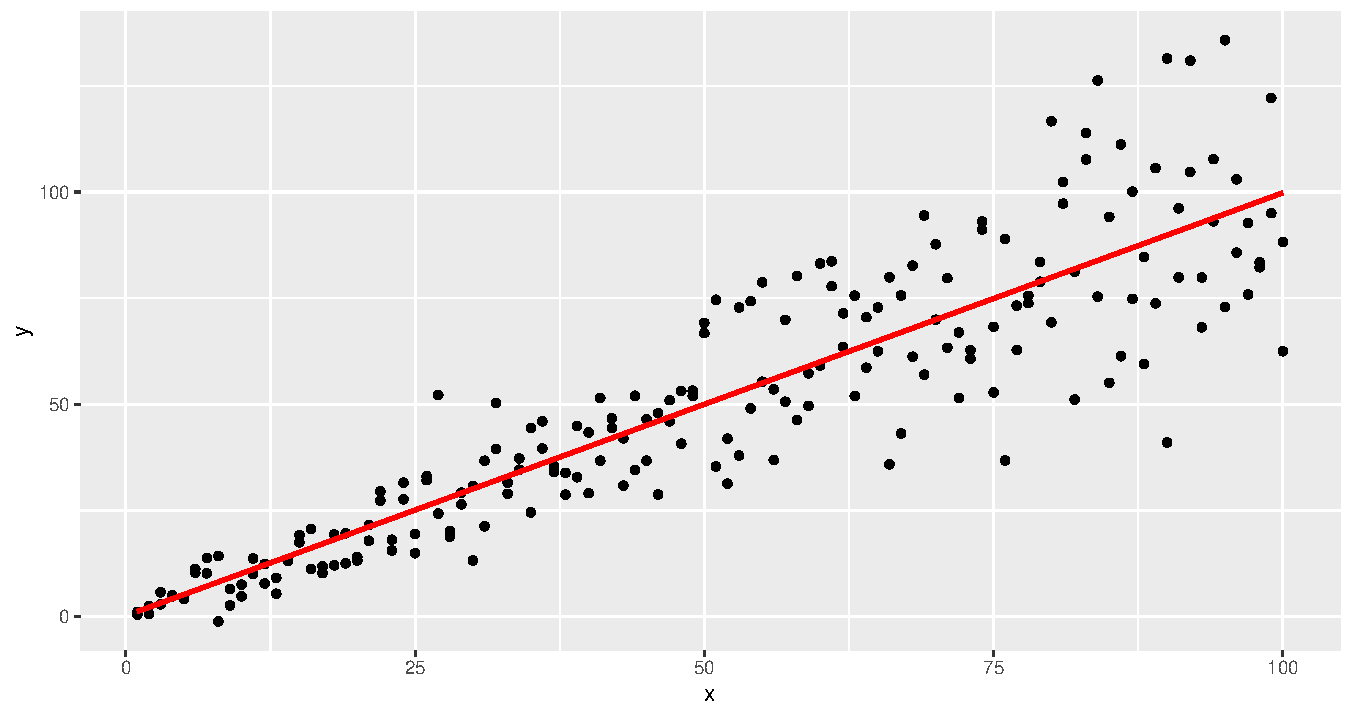
\includegraphics[width=110mm]{pictures/week_18_het_1.pdf}
\end{figure}
\end{frame}

\begin{frame}
\frametitle{Heteroscedasticity: visualization}
\begin{figure}
\centering
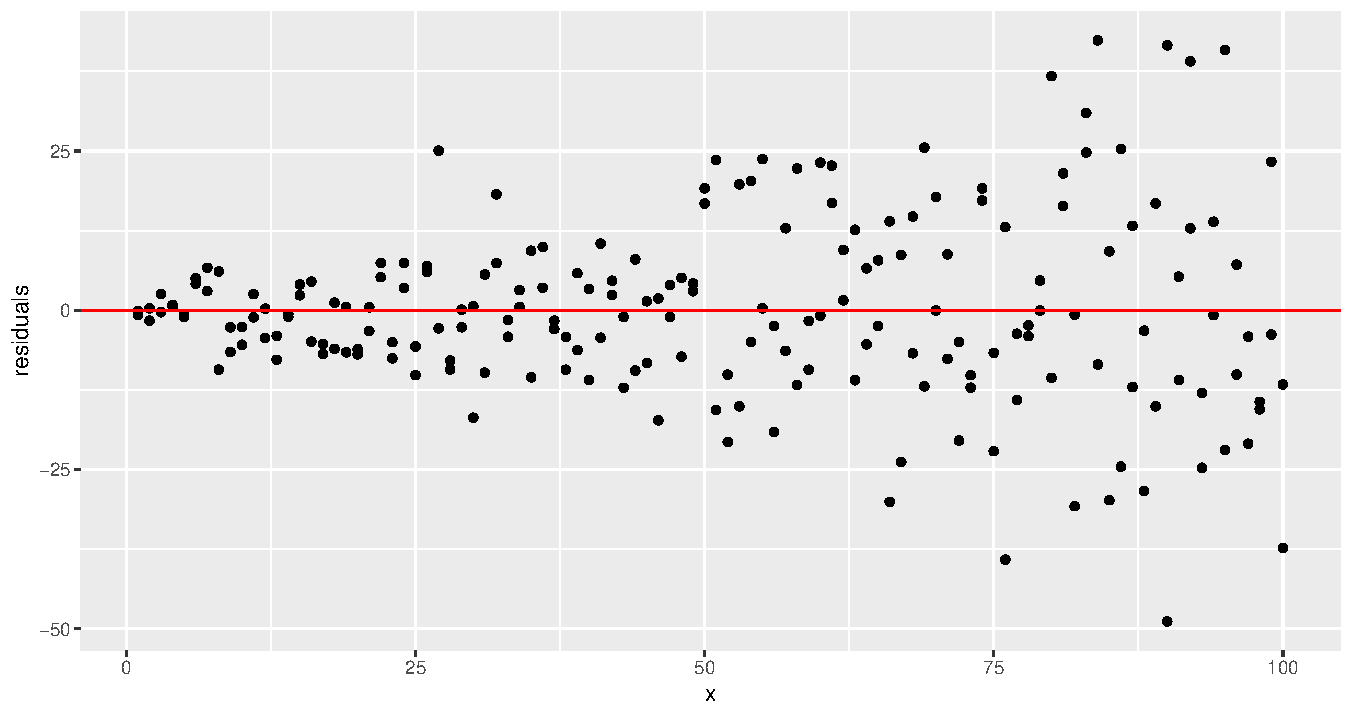
\includegraphics[width=110mm]{pictures/week_18_het_2.pdf}
\end{figure}
\end{frame}

\begin{frame}
\frametitle{Heteroscedasticity}
Let's start with fixing heteroscedasticity:
\begin{itemize}
\item Heteroscedasticity means that the variance of the disturbances, $\sigma^2$, in our sample is not constant. \pause
\item Assumption 5,  $Var(u|\mathbf{X})=\sigma^2$, is violated and we cannot replace the population variance $Var(u|\mathbf{X})$ by $\hat{\sigma}^2=\frac{\mathbf{\hat{u}'\hat{u}}}{N-K-1}$ \pause
\item We can use \textbf{robust standard errors} to allow for such violation
\item[] (while still assuming \textbf{no} serial correlation/autocorrelation) \pause
\item We \textbf{estimate} the covariance matrix $\Sigma=E(\mathbf{\hat{u}}\mathbf{\hat{u}}'|\mathbf{X})$ using $\hat{\Sigma}$
\end{itemize}
\[\hat{\Sigma}=
\left[
\begin{array}{cccc}
\hat{u}^2	& 0			& \ldots	& 0\\
0 			& \hat{u}^2 & \ldots	& 0\\
\vdots 		& \vdots	& \ddots 	& \vdots\\
0 			& 0			& \ldots	& \hat{u}^2 
\end{array}
\right]
\]

\end{frame}


\begin{frame}
\frametitle{White-robust estimators}
\begin{itemize}
\item We use residuals of the prediction of $y_i$ \textbf{by our model} for each $i$ \pause
\item Purely empirical solution \pause
\item White has proved that the diagonal of matrix $\hat{\Sigma}$ is a consistent but biased estimator of $\Sigma=E(\mathbf{\hat{u}}\mathbf{\hat{u}}'|\mathbf{X})$ in small samples \pause
\item Your statistical software will multiply the squared residuals of each $i$ by $n/df=n/(n-k-1)$ as a degree of freedom correction to have unbiased estimates \pause
\item The estimate of the variance of the OLS estimator becomes
$$\widehat{Var}(\mathbf{\hat{\beta}})=\frac{n}{df}(\mathbf{X'X})^{-1} \mathbf{X}' \hat{\Sigma} \mathbf{X} (\mathbf{X}'\mathbf{X})^{-1}$$
\item This robust variance estimator is called \textbf{Sandwich estimator} giving us \textbf{White-Huber standard errors}
\end{itemize}
\end{frame}

\begin{frame}
\frametitle{Robust estimation in \texttt{R}}
Using \texttt{R} today we will:
\begin{enumerate}
\item Compute OLS and estimates of the S.E. using \texttt{lm()} and matrix algebra
\item Represent heteroscedasticity
\item Compute White-robust estimators for S.E. using \texttt{vcovHC()}, matrix algebra and \texttt{lm\_robust()}
\item Perform a Breusch-Pagan test on heteroscedasticity
\end{enumerate} \pause

We are not doing it in Stata today, cause matrix algebra is definitely less handy\ldots Equivalent commands exist, yet:
\begin{itemize}
\item To estimate robust standard errors: \texttt{reg ..., robust}
\item To perform a Breusch-Pagan test: \texttt{estat hettest}
\item To visualise heteroscedasticity after a regression: \texttt{rvfplot}
\end{itemize}
\end{frame}

\begin{frame}
\frametitle{Serial correlation (time, space, both)}
Now, serial correlation: 
\begin{itemize}
\item Observations may be related within groups (e.g., within individuals, states, countries, within a unit across time periods). Typical problem with time series, spatial correlation, panel data \pause
\item With $i \neq j$,
\[E[u_{(i)g},u_{(j)g'}] = 
	\begin{cases} 
		0\qquad\quad\text{if}\,g=g'\\
		\sigma_{(ij) g}\quad\,\text{if}\,g\neq g'
	\end{cases}
\]
\end{itemize}
\end{frame}

\begin{frame}
\frametitle{Clustered observations}
\begin{itemize}
\item Say, we have individuals clustered in $G$ groups with $N_g$ \pause
\[ Var(\mathbf{b}|\mathbf{X}) = E \left[(\mathbf{X}'\mathbf{X})^{-1}\mathbf{X}'\Sigma\mathbf{X}(\mathbf{X}'\mathbf{X})^{-1}\right]
\]
\item with $\Sigma$ given by
\end{itemize}
\footnotesize
\vspace{.3cm}
\[
\left[
\begin{array}{ccccccccc}
\sigma^2_{(11)1} & \ldots & \sigma^2_{(1N_1)1} & 0 & \ldots & 0 & 0 & \ldots & 0\\
\vdots & \ddots & \vdots & \vdots & \ddots & \vdots & \vdots & \ddots & \vdots\\
\sigma^2_{(N_11)1} & \ldots & \sigma^2_{(N_1N_1)1} & 0 & \ldots & 0 & 0 & \ldots & 0\\
0 & \ldots & 0 & \sigma^2_{(11)2} & \ldots & \sigma^2_{(1N_2)2} & 0 & \ldots & 0 \\
\vdots & \ddots & \vdots & \vdots & \ddots & \vdots & \vdots & \ddots & \vdots \\
0 & \ldots & 0 & \sigma^2_{(N_21)2} & \ldots & \sigma^2_{(N_2N_2)1} & 0 & \ldots & 0 \\
0 & \ldots & 0 & 0 & \ldots & 0 & \sigma^2_{(11)G} & \ldots & \sigma^2_{(1N_G)G} \\
\vdots & \ddots & \vdots & \vdots & \ddots & \vdots & \vdots & \ddots & \vdots \\
0 & \ldots & 0 & 0 & \ldots & 0 & \sigma^2_{(N_G1)G} & \ldots & \sigma^2_{(N_GN_G)G}\\
\end{array}
\right]
\]
\normalsize
\end{frame}

\begin{frame}
\frametitle{Dealing with clustered observations}
What to do? We need an estimator for the variance that accounts for clustering: 
\begin{itemize}
\item We practically never know $\sigma^2_{(N_gN_g)g}$: we need an estimate \pause
\item We will use the residuals: the amount by which the prediction $\mathbf{\hat{y}=X\beta}$ is off from the actual values of $\mathbf{y}$, \pause \textbf{but now} computed separated \textit{within} each cluster of observations: \pause
\begin{equation}
\frac{\sum\limits_{i=1}^{N_g}{\hat{u}_i}^2}{N_g}, \quad i\in g
\end{equation}
\pause
\item[] or $\mathbf{\hat{u}_g'\hat{u}_g}/N_g$ where the numerator is SSR for all observations within each cluster.
\end{itemize}
\end{frame}

\begin{frame}
\frametitle{Robust estimation and GLS}
We can do even better:
\begin{itemize}
\item \textbf{Robust standard errors} use a robust covariance matrix. Keep the coefficient estimate but adjust \textbf{standard errors} to account for the violation of the assumption of i.i.d. $\rightarrow$ we get a conservative estimate!
\item \textbf{Generalized least squares} proceed in two stages. First estimate the covariance matrix (stage 1) and then adjust coefficients (stage 2) $\rightarrow$ GLS may be more efficient
\end{itemize}
\end{frame}

\begin{frame}[fragile]
\frametitle{Generalized Least Squares (GLS)}
\begin{itemize}
\item A family of estimators that generalise OLS procedures (OLS become only a particular case). \pause
\item Weighted Least Squares (WLS):
\item[] $\mathbf{\hat{\beta}}= (\mathbf{X'} \textcolor{ForestGreen}{diag \left[ \mathbf{W} \right]} \mathbf{X})^{-1}\mathbf{X}' \textcolor{ForestGreen}{diag \left[ \mathbf{W} \right]} \mathbf{Y}$ \pause
\item You can use WLS with heteroscedasticity because you give a higher weight to data points with a smaller error variance, cause they are more informative! \pause
\item You just need to specify the correct weight matrix $\mathbf{W}$
\item One common choice is to use the inverse of the OLS residuals (stage 1) as $\mathbf{W}$ for WLS (stage 2). \pause In this case we have Feasible Last Squares (FGLS)
\item See an example in \texttt{R}
\end{itemize}
\end{frame}

\begin{frame}
\frametitle{Take away points}
\begin{enumerate}
\item \textbf{Always use robust standard errors!!!}
\item Consider whether your observations are clustered in a meaningful way, if yes, use clustered standard errors
\item Consider GLS as further robustness check on your estimation but (1) and (2) are mostly good enough. 
\item R and Stata feature plenty of ways to implement robust and clustered standard errors; know how they work. 
\end{enumerate}
\end{frame}

\section{Non-parametric tests}

\frame{
\frametitle{Introduction}
\begin{itemize}
\item There are alternatives to the t-test and F-test
\item Choose your test based on your problem, and not the other way around
\item Do not stick to parametric tests if your problem requires you to do otherwise
\end{itemize}
}

\begin{frame}
\frametitle{Pick an appropriate (non-parametric) test}
\begin{enumerate}
\item Intro to non-parametric tests
\item Success probability: binomial test
\item Tests of differences between groups -- paired from one-sample and independent from two-sample
\begin{itemize}
	\item Fisher sign test and Wilcoxon sign-rank test
	\item Comparing success probabilities: Fisher's exact test
\end{itemize}
%\item Alternatives to correlation coefficients \pause -- bivariate relationships 
%\begin{itemize}
%	\item Spearman's $\rho$
%	\item Kendall's $\tau$
%\end{itemize}
\end{enumerate}
\end{frame}

\begin{frame}
\frametitle{What are non-parametric tests}
Non-parametric tests: 
\begin{itemize}
\item Make fewer assumptions about the population -- \textbf{distribution-free} tests \pause 
\item Are more robust to outliers and heterogeneity of variance \pause
\item Are robust even if you cannot reasonably characterize the distribution of the underlying population \pause
\item Are applicable for interval and ordinal data -- some even for nominal data \pause
\item Have test statistics that are distributed normally when N is large
\end{itemize}
\end{frame}

\begin{frame}
\frametitle{When are non-parametric tests advantageous}
\begin{itemize}
\item When assumptions of parametric tests/estimators are not met. Example: t-statistic is not t-distributed if underlying population not normal or sample size too small \pause
\item Often easier to compute manually than their parametric alternatives \pause
\item We can often derive the exact distribution of the test statistic
\end{itemize}
\end{frame}

\begin{frame}
\frametitle{Disadvantages of non-parametric tests}
\begin{itemize}
\item Mostly no estimates of variance \pause
\item Mostly no confidence intervals \pause
\item Need more observations to draw a conclusion with same certainty \pause i.e., less powerful as parametric alternative when assumptions for parametric tests are met \pause
\item \textbf{Yet} often differences are small, and parametric alternatives perform vastly worse when assumptions are not met 
\end{itemize}
\end{frame}

\begin{frame}
\frametitle{Binomial test: Basics}
\begin{itemize}	
\item Observing outcome $B$ of $n$ independent repeated Bernoulli trials, can I say that success probability for each trial $p=p_0$? $P(p_0|B,n)$? \pause Example: you toss 5 times a coin and count the number of Heads. You get Heads = 3. Can we say $p=.5$? \pause
\item Assumptions:
\begin{enumerate}
	\item Dichotomous data: outcomes are success or failure
	\item $p$ remains constant for each trial
	\item $n$ trials are independent
\end{enumerate}
\item $H_0: p = p_0$ \pause
\item Other tests/statistics below relate to the basic binomial test of significance \pause
\item Under assumptions 1-3, it is a distribution-free test of $H_0$ because the probability distribution of $B$ is determined without further assumptions on the distribution of the underlying population
\end{itemize}
\end{frame}

\begin{frame}
\frametitle{Binomial test: Procedure}
\begin{itemize}	
\item To test $H_0: p = p_0$ we set the desired level of significance $\alpha$ and we set $B$ to number of observed successes with $n$ trials \pause
\item Build the binomial distribution under the null-hypothesis \pause
\item Reject $H_0$ if $B\geq b_{\alpha_{2}}$ or $B\leq b_{\alpha_{1}}$ \pause
\item Where $b_{\alpha_{2}}$ is the upper $\alpha_2$ percentile point and $b_{\alpha_{1}}$ is the lower $\alpha_1$ percentile point with $\alpha = \alpha_1 + \alpha_2$ 
\end{itemize}
\end{frame}

\begin{frame}
\frametitle{Binomial test: Example}
\begin{itemize}	
\item Say $n=8$ and we test $H_0:p=.4$ vs $H_1: p\neq.4$\pause
\item You can use the table of the binomial distribution or your statistical software and quantile function to obtain the binomial distribution for $n=8$ and $p=.4$. Suppose that $\alpha=.05$. Under the null-hypothesis the distribution: \pause
	\begin{itemize}
	\item[--] leaves $2.5\%$ of the observations to the left of 1
	\item[--] leaves $2.5\%$ of the observations to the right of 6
	\end{itemize}
\item We reject $H_0: p = .4$ if 6 or more successes are observed as well as if 1 or less successes are observed 
\end{itemize}
\end{frame}

\begin{frame}{Sign test (Fisher): Basics}
\begin{itemize}
\item Alternative to paired t-test (\emph{e.g.} difference-in-means) which assumes normality and equal variance across groups in underlying data \pause
\item Information taken from \textbf{signs} in difference between paired observations \pause
\item Assumptions: \pause
	\begin{itemize}
	\item[--] paired observations $(X_1^1,X_1^2),\ldots,(X_N^1,X_N^2$) are \textbf{random} sample and iid
	\item[--] paired observations are dependent
	\item[--] paired differences come from same continuous distribution
	\end{itemize} \pause
\item Use when \textbf{direction} of difference between two measurements on same unit can be determined
\end{itemize}
\end{frame}

\begin{frame}{Sign test: Procedure}
\begin{itemize}
\item Compute differences $D_i = X_i^1 - X_i^2$ between $N$ pairs of matched observations. 
\item Count the number of positive and negative $D_i$, $n^+$ and $n^-$. \textbf{We do not care about their size!} \pause
\item If there is no difference in the samples, then the median of the distribution of $D_i$, $\theta$, should be 0. $H_0:\theta = 0$ vs $H_1:\theta>0$. \pause
\item $n^+$ is our test statistic. What is its distribution? It's binomial if we consider ``being positive'' as a Bernoulli random variable! \pause
%\item Under $H_0$ number of positive and negative differences should be equal. \pause
\item Calculate the binomial coefficient $B={N\choose n^+}$. $B/2^N$ is the probability of getting \textbf{exactly} the amount of $n^+$ and $n^-$ under the null.
\item To get a p-value, sum all binomial coefficients that are $\leq B$ and divide by $2^N$
\end{itemize}	
\end{frame}

\begin{frame}[fragile]{Sign test: Example}
\begin{itemize}
\item Consider the table below. (\texttt{income}-variable in \texttt{gssData.dta}) \pause
\item Question: Did income increase from '08 to '12?
\item Note, it is an ordinal measured variable, taking a difference may not make sense -- assume for this example that it does \pause
\end{itemize}
	
\begin{verbatim}
     +---------------------------+
     | income08   income12   D_i |
     |---------------------------|
  1. |        3         19   -16 |
  2. |        4          9    -5 |
  3. |       17         20    -3 |
  4. |       15         17    -2 |
  5. |       14         16    -2 |
  ...
\end{verbatim}
\end{frame}


\begin{frame}{Sign test: Example}
\begin{itemize}
\item Differences: \pause -10 -9 -8 -6 -4 -4 -3 0 \textbf{1 1 2 2 3 5 16} \pause
\item How likely is it to observe 7 positive $D_i$ when $H_0: \theta=0$ is true, thus with no difference between income in 2008 and 2012? \pause
$$B={N\choose n^+}=\frac{15!}{8! 7!}=6435$$
\item Thus we have that the probability of getting exactly 7 positive differences is $B/2^N=6435/2^{15}=0.19$
\item To get the related p-value we should sum all binomial coefficients that are $\leq B$ and divide the sum by $2^N$. \pause
\item We can do quicker: What is the distribution of $D_i$? \pause
\item Binomial with $N=15$, $p=.5$ (under $H_0$), and $x=7$. \pause
\item Our p-value is $Prob(X\leq 7) = 0.50$ \pause
\item Statistical packages will then compute these for you
\end{itemize}	
\end{frame}

\begin{frame}{Sign test: Small sample issues}
\begin{itemize}
\item Only needs \textbf{sign} of difference, not difference itself \pause
\item Less efficient than Wilcoxon sign-rank test (uses only sign not ordering) but rather robust to outliers \pause
\item How to deal with $D_i=0$? Usually ignored but reduces effective sample size \pause
\item Works for interval data but pay attention to ties - which correction for tied values?
\end{itemize}
\end{frame}

\begin{frame}{Wilcoxon sign-rank test: Basics}
\begin{itemize}
\item Alternative to paired t-test which assumes normality and equal variance across groups in underlying data \pause
\item Information taken from signs in difference between paired observations (pre- vs post-treatment)\pause
\item When actual difference pre- vs post-treatment is greater than 0, tendency to larger proportion of positive differences
\end{itemize}
\end{frame}

\begin{frame}{Wilcoxon sign-rank test: Basics}
\begin{itemize}
\item Assumptions: \pause 
	\begin{itemize}
	\item paired observations $(X_1^1,X_1^2),\ldots,(X_N^1,X_N^2)$ are random sample and iid \pause i.e., differences are mutually independent (while paired observations are dependent)\pause
	\item paired differences come from a continuous distribution \pause
	\end{itemize}
\item Test of null hypothesis of zero shift in location (no treatment effect), $H_0:\theta=0$ -- null hypothesis states that each of the distributions for the differences is symmetrically distributed around the 0 \pause
\item Use when direction of difference \textbf{and magnitude} between two measurements on same unit can be determined
\end{itemize}

\end{frame}


\begin{frame}{Wilcoxon sign-rank test: Procedure}
\begin{itemize}
\item Compute difference $D_i = X_i^1 - X_i^2$ between $N$ pairs of matched observations	
\item Order \textbf{absolute values} of differences from smallest to largest \pause
\item Let $S_i$ denote the rank of $D_i$ in the joint ordering (assign average rank to ties) \pause
\item ``Wilcoxon signed rank statistic'', $W^+$, is sum of positive signed ranks 
\item Under $H_0: \theta =0$, $W^+$ is distributed according to the distribution derived by Wilcoxon (1954)
\item Reject $H_0$ if $W^+\geq w_{\alpha/2}$ or $W^+\leq\frac{N(N+2)}{2}-w_{\alpha/2}$
\item distribution of W is based on permutations of all possible rankings
\end{itemize}
\end{frame}

\begin{frame}[fragile]{Wilcoxon sign-rank test: Example}
$N=15$
\begin{verbatim}
     +-------------------------------------------+
     | income08   income12   D_i   absD_i   rank |
     |-------------------------------------------|
  1. |       22         22     0        0      1 |
  2. |       20         21    -1        1    2.5 |
  3. |       20         21    -1        1    2.5 |
  4. |       14         16    -2        2    4.5 |
  5. |       15         17    -2        2    4.5 |
     |-------------------------------------------|
  6. |       16         13     3        3    6.5 |
  7. |       17         20    -3        3    6.5 |
  8. |       21         17     4        4    8.5 |
  ...
\end{verbatim}
\end{frame}


\begin{frame}{Wilcoxon sign-rank test: Distribution of $W^+$}
\begin{itemize}
\item Sum of ranks of positive differences: 74.5 (Sum of ranks of negative difference: 45.5) \pause
\item Lowest possible sum of ranks of positive differences? \pause $0$ -- no absolute value of differences is positive \pause
\item Highest possible? $N(N+1)/2 = 15(16)/2 = 120$ -- all differences are positive \pause
\item What is the smallest significance level at which these data lead to rejection of $H_0$? \pause
\item Consulting statistical tables of $W^+$ distribution, for our example we have $N=14$ and $W^+=74.5$ 
\end{itemize}
\end{frame}

\begin{frame}{Critical values of $W^+$ for $N=14$. Hollander/Wolfe, p.576}
\begin{figure}[H]\centering
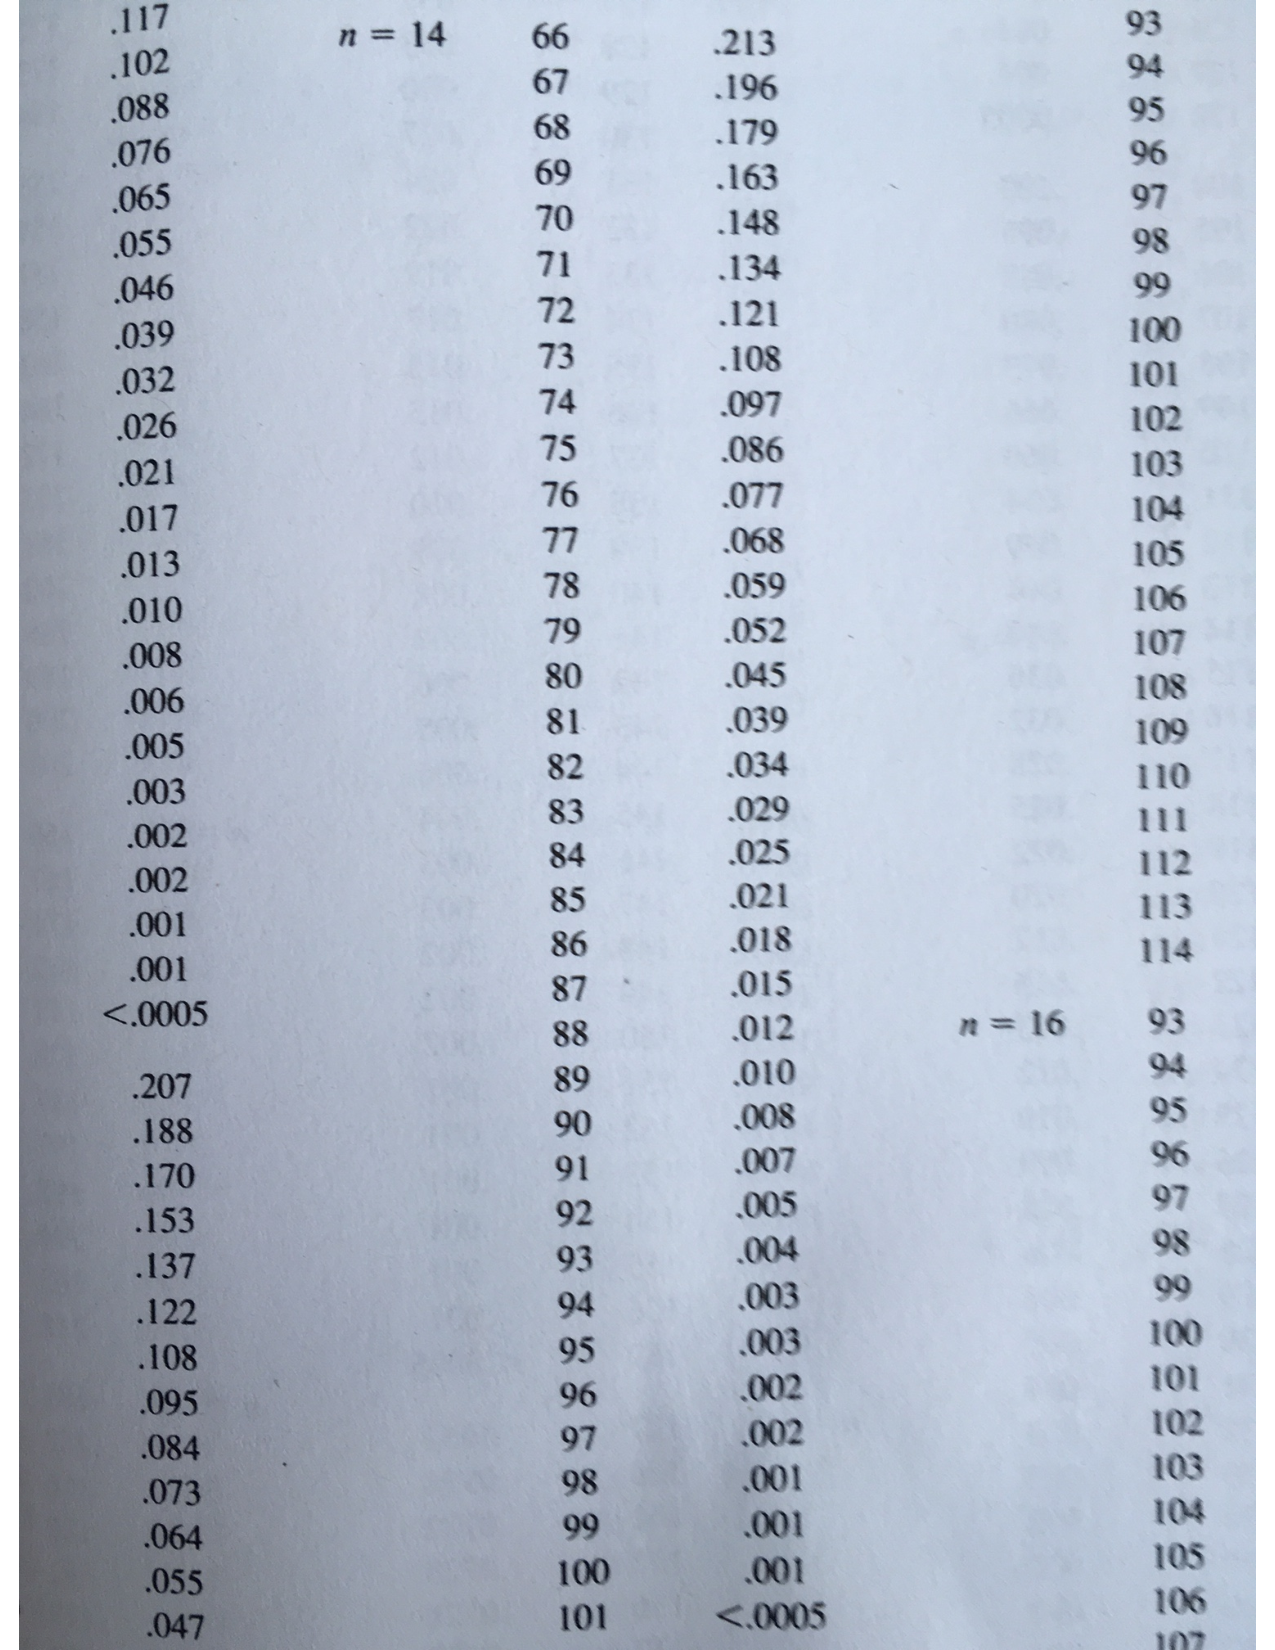
\includegraphics[scale=.27]{pictures/wilcoxonRankSignTableN14.pdf}
\end{figure}
\end{frame}

\begin{frame}{Wilcoxon sign-rank test: Example}
\begin{itemize}
\item Reject $H_0$ if $W^+\geq w_{\alpha/2}$ or $W^+\leq\frac{n(n+2)}{2}-w_{\alpha/2}$ \pause
\item For $\alpha=.052$, reject if $W^+ \geq 80$ or $W^+\leq\frac{15(16)}{2} - 80 = 120 - 80 = 40$ \pause -- so we do not reject \pause
\item Large sample approximation: \pause
	\begin{itemize}
	\item[--] Standardize $W^+$: Under the null, $E(W^+)=\frac{n(n+1)}{4}$ and $var(W^+)=\frac{n(n+1)(2n+1)}{24}$ \pause
	\item[--] $W^* = \frac{W^+ - E(W^+)}{\sqrt{var(W^+)}}$ \pause
	\item[--] With $n\rightarrow\infty,\,W^+\sim N(0,1)$ \pause
	\item[--] Adjustments for ties are needed
	\end{itemize}
\item Your statistical package will perform this test for you, but this is what happens under the surface
\end{itemize}
\end{frame}

\begin{frame}{Wilcoxon sign-rank test: Small sample issues}
\begin{itemize}
\item Wilcoxon sign-rank test incorporates more information than Fisher's sign-test but also needs more information \pause
\item How to deal with $D_i=0$? Usually ignored but reduces effective sample size \pause
\item Works for interval data but pay attention to ties - which correction for tied values?
\end{itemize}
\end{frame}

\frame{
\frametitle{Fisher's exact test -- Intuition}
When do we use it?
\begin{enumerate}
\item When we have two independent samples arranged in a contingency table
\item When in each sample we measure the frequency of success \emph{vs} failure (Bernoulli)
\item When expected frequency of any success or failure is below 5. Otherwise use $\chi^2$ test
\end{enumerate}
}

\frame{
\frametitle{Fisher's exact test -- Three cases}
\begin{enumerate}
\item Row totals are fixed, column totals are random (or the other way around) \pause
	\begin{itemize}
	\item The hypothesis tested is $p_1 = p_2$ \pause
	\end{itemize}
\item Both row totals and column totals are random \pause
	\begin{itemize}
	\item The hypothesis tested is bivariate independence \pause
	\end{itemize}
\item Both row totals and column totals are fixed \pause
	\begin{itemize}
	\item The hypothesis tested is independence
	\end{itemize}
\end{enumerate}
}

\frame{
\frametitle{Fisher's exact test -- Basics}
\begin{enumerate}
\item indicate as $O_{1S}$ the \emph{S}uccessful outcome you observe from sample 1 (similarly you have $O_{1F}$, $O_{2S}$, $O_{2F}$).
\item Indicate as $n_{1\cdot}$ ($n_{2\cdot}$) the independent repeated Bernoulli trials from sample 1 (2), each one with success probability $p_1$ ($p_2$)
\end{enumerate}
We will have:
\begin{tabular}{l|cc|c}
			& Successes 	& Failures 		& Totals\\
\hline
Sample 1	& $O_{1S}$		& $O_{1F}$ 		& $n_{1\cdot}$ \\
Sample 2	& $O_{2S}$		& $O_{2F}$ 		& $n_{2\cdot}$ \\
\hline
Totals		& $n_{\cdot S}$	& $n_{\cdot F}$ 	& $n$ \\
\end{tabular}

\begin{center}
$H_0: p_1 = p_2 = p$ \\
$H_1: p_1 \neq p_2$
\end{center}
}

\frame{
\frametitle{Fisher's exact test -- Procedure}
\begin{itemize}
\item In effect the test asks ``what is the probability of having a table as extreme as the one we observe, if the null hypothesis is true''?
\item Hypergeometric distribution: $Prob(O_{1S}=x|n_{1\cdot},n_{2\cdot},n_{\cdot S},n_{\cdot F}) = \frac{n_{1\cdot}!n_{2\cdot}!n_{\cdot S}!n_{\cdot F}!}{n! x! O_{1F}!O_{2S}!O_{2F}!}$
\item Fisher's exact test rejects $H_0: p_1=p_2$ if your observed $O_{1S}\geq q_{\alpha}$
\item Where $q_{\alpha}$ is chosen from the conditional distribution described above so that $Prob(O_{1S}=q_{\alpha}|n_{1\cdot},n_{2\cdot},n_{\cdot S},n_{\cdot F})=\alpha$ where $\alpha$ is our desired level of significance 
\end{itemize}
}

\frame{
\frametitle{Fisher's exact test -- Examples}
Suppose you are curing two independent samples of patients, one gets an innovative drug and the other gets the traditional one. You measure success as cure, failure as not cure
\begin{center}
\begin{tabular}{l|cc|c}			& S (cured) 	& F (not cured)	& Totals\\
\hline
S1 (new drug)	& 5				& 4		 		& 9 \\
S2 (old drug)	& 4				& 2		 		& 6 \\
\hline
Totals		& 9				& 6			 	& 15 \\
\end{tabular}
\end{center}

\begin{itemize}
\item Assume horizontal and vertical totals are fixed
\item $H_0: p_1<p_2$
\item Under the null-hypothesis, what are the probabilities of the tables that would give us a value as small as or smaller than the observed value of $O_{1S}=5$?
\end{itemize}
}

\frame{
\frametitle{Fisher's exact test -- Example}
\begin{table}
\centering
\resizebox{\columnwidth}{20pt}{%
\begin{tabular}{c| ccc ccc ccc ccc ccc ccc cc}
Sample 1 & 3 & 6 && 4 & 5 && 5 & 4 && 6 & 3 && 7 & 2 && 8 & 1 && 9 & 0\\
Sample 2 & 6 & 0 && 5 & 1 && 4 & 2 && 3 & 3 && 2 & 4 && 1 & 5 && 0 & 6\\
p & \multicolumn{2}{c}{.017} && \multicolumn{2}{c}{.151} && \multicolumn{2}{c}{.378} && \multicolumn{2}{c}{.336} && \multicolumn{2}{c}{.108} && \multicolumn{2}{c}{.011} && \multicolumn{2}{c}{.000}\\
\end{tabular}%
}
\end{table}

\begin{itemize}
\item $H_0: p_1<p_2$
\item Under the null-hypothesis, what are the probabilities of the tables that would give us a value as small as or smaller than the observed value of $O_{1S}=5$?
\item It will be $p=.017+.151+.378=.546$
\end{itemize}
}

\frame{
\frametitle{Fisher's exact test -- Example}
If (with the same horizontal and vertical totals) what we observe were:
\begin{center}
\begin{tabular}{l|cc|c}			& S (cured) 	& F (not cured)	& Totals\\
\hline
S1 (new drug)	& 8				& 1		 		& 9 \\
S2 (old drug)	& 1				& 5		 		& 6 \\
\hline
Totals		& 9				& 6			 	& 15 \\
\end{tabular}
\end{center}

The probability of having a table as extreme (or more) as the one you observe  would be: $p=0.0107+0.0002=0.0109$ ! 
}


\frame{
\frametitle{Conclusion}
\begin{center}
All clear? Questions? \\
Thanks and see you next week!
\end{center}
}

\end{document}